
\documentclass{report}

\usepackage{amsmath}
\usepackage{amssymb}
\usepackage{cite}
\usepackage{titlepic}
\usepackage{graphicx}
\usepackage{url}
\usepackage{xfrac}
\usepackage{tabto}
\usepackage{caption}
\usepackage{nameref}
\usepackage{csquotes}
\usepackage{float}

\NumTabs{10}
\graphicspath{{./images/}}
\setlength\parindent{0pt}
\NewDocumentCommand{\chapref}{s m}{Chapter~\ref{#2}\IfBooleanF{#1}{ (\nameref{#2})}}

\DeclareMathOperator{\erf}{erf}





\begin{document}






\titlepic{
\includegraphics[scale=0.5]{DIT_logocol}}
\title{The Problem with Continuous Casting}
\author{Jerry Kiely\\
  \\
  School of Mathematical Sciences\\
  Dublin Institute of Technology\\
  Dublin 8\\
  \\
  \texttt{d16126734@mydit.ie}}
\date{\today}
\maketitle







\tableofcontents







\begin{abstract}
In this paper we will write a mathematical model for the continuous casting process in order to 
evaluate it's  feasibility for producing steel sheets of varying thickness. We will initially discuss 
\emph{moving boundary problems}, followed by \emph{The Stefan Condition}. We will then discuss a simpler 
problem relating to a freezing boundary before moving on to the industrial problem. We will then discuss 
our results and evaluate the feasability of the approach.
\end{abstract}







\chapter{Introduction}










\section{Moving Boundary Problems}

John Crank describes \emph{Moving boundary problems} as\bigskip

\begin{displayquote}
associated with time-dependent problems, and the position of the boundary has to be determined as a 
function of time and space~\cite{crank1987free}
\end{displayquote}\medskip

Also known as Stefan problems, these are problems where the (physical) boundary can change, or move, 
with time. These problems often occur in the context of phase changes - where a substance transitions 
from solid to liquid, or from liquid to gas - i.e. problems that involve:\bigskip

\begin{itemize}

\item evaporation

\item condensation

\item melting

\item solidification

\end{itemize}\medskip

In the context of these kinds of problems, an amount of heat energy is either required or released in order 
to transition from one phase to another: in the case of solidification / melting, the heat required to melt 
a substance is called the \emph{latent heat of fusion}, and in the case of evaporation / condensation, the 
heat required to evaporate a substance is called the \emph{latent heat of vaporisation}. We usually talk 
about the \emph{specific latent heat} of a substance, denoted $\lambda$, which is the latent heat per unit 
mass of the substance.\bigskip











\section{The Stefan Condition}

Stefan conditions deal with the boundary between two phases of a substance, such as ice and water, or water 
and steam. We will now derive a boundary condition to capture this evolving physical boundary.\bigskip

Let us consider a (physical) boundary between ice and water as it freezes, and with an advancing frozen 
boundary. By applying conservation of energy we can say that the heat released by water as it freezes is 
equal to the the heat removed from the region by conduction. We consider that the boundary will advance 
$\delta s$ in a period $\delta t$. Hence, the mass that solidifies in the time $\delta t$ is:\bigskip

\begin{eqnarray*} 
  m_{sol} & = & \rho A (s(t + \delta t) - s(t)) \\
          & = & \rho A \delta s
\end{eqnarray*}\medskip

where $\rho$ is the density of water, and $A$ is the cross-sectional area of the boundary. Thus the heat 
released in the period $\delta t$ is:\bigskip

\begin{eqnarray*} 
  H_{sol} & = & \lambda m_{sol} \\
          & = & \lambda \rho A \delta s
\end{eqnarray*}\medskip

where $\lambda$ is the specific latent heat of fusion of water. We can assume that the water temperature 
is uniform, that the ice is colder than the water, and thus the heat released is conducted back through 
the ice. The amount of heat that flows across the boundary is therefore the heat flux multiplied by the 
cross-sectional area of the boundary. The heat flux is:\bigskip

\[ J = -k \frac{\partial u}{\partial x} \]\medskip

so the heat conducted back through the ice in the period $\delta t$ is:\bigskip

\begin{eqnarray*} 
  H_{con} & = & -J A \delta t \\\\
          & = & k \frac{\partial u}{\partial x} (s(t), t) A \delta t
\end{eqnarray*}\medskip

where the negative value denotes the heat movement in the negative $x$ direction. By equating both the 
heat released by solidification and the heat conducted back through the ice we get the following:\bigskip

\begin{eqnarray*} 
  k \frac{\partial u}{\partial x} (s(t), t) A \delta t & = & \lambda \rho A \delta s \\\\
             k \frac{\partial u}{\partial x} (s(t), t) & = & \lambda \rho \frac{\delta s}{\delta t}
\end{eqnarray*}\medskip

In the limit as $\delta t \to 0$, $\delta s \to 0$, and the equation becomes:\bigskip

\[ k \frac{\partial u}{\partial x} (s(t), t) = \lambda \rho \frac{d s}{d t} \]\medskip











\section{Similarity Solution For The Heat Equation}

We will now look for a general solution for the 1-D heat equation:\bigskip

\begin{eqnarray*} 
  \frac{\partial u}{\partial t} & = & \alpha \frac{\partial^2 u}{\partial x^2} \\\\
                        u(x, 0) & = & 0 \\
                        u(0, t) & = & u_0 \\
                   u(\infty, t) & = & 0 
\end{eqnarray*}\medskip

To begin with, let us assume that the solution can be expressed as a function of both $x$ and $t$ in the 
following way:\bigskip

\[ u(x, t) = f(z) \]\medskip

where $z$ is a function of both $x$ and $t$:\bigskip

\[ z = \frac{x}{\sqrt{\alpha t}} \]\medskip

This will allow us to transform the equation into a simpler form. Starting with the first derivative of 
$u$ with respect to $t$:\bigskip

\begin{eqnarray*} 
    \frac{\partial u}{\partial t} & = & \frac{\partial f(z)}{\partial t} \\\\
                                  & = & \frac{\partial f(z)}{\partial z} \cdot \frac{\partial z}{\partial t} \\\\
                                  & = & f'(z) \cdot \left( \frac{-x \alpha}{2} \right) \cdot (\alpha t)^{\sfrac{-3}{2}} 
\end{eqnarray*}\medskip

followed by the first derivative of $u$ with respect to $x$:\bigskip

\begin{eqnarray*} 
    \frac{\partial u}{\partial x} & = & \frac{\partial f(z)}{\partial x} \\\\
                                  & = & \frac{\partial f(z)}{\partial z} \cdot \frac{\partial z}{\partial x} \\\\
                                  & = & \frac{f'(z)}{\sqrt{\alpha t}}
\end{eqnarray*}\medskip

and finally the second derivative of $u$ with respect to $x$:\bigskip

\begin{eqnarray*} 
\frac{\partial^2 u}{\partial x^2} & = & \frac{\partial}{\partial x} \left( \frac{\partial u}{\partial x} \right) \\\\
                                  & = & \frac{\partial}{\partial x} \left( \frac{f'(z)}{\sqrt{\alpha t}} \right) \\\\
                                  & = & \frac{1}{\sqrt{\alpha t}} \cdot \frac{\partial f'(z)}{\partial x} \\\\
                                  & = & \frac{1}{\sqrt{\alpha t}} \cdot f''(z) \cdot \frac{\partial z}{\partial x} \\\\
                                  & = & \frac{1}{\sqrt{\alpha t}} \cdot f''(z) \cdot \frac{1}{\sqrt{\alpha t}} \\\\
                                  & = & \frac{f''(z)}{\alpha t} 
\end{eqnarray*}\medskip

Substituting the above into the heat equation we get:\bigskip

\begin{eqnarray*} 
f'(z) \cdot \left( \frac{-x \alpha}{2} \right) \cdot (\alpha t)^{\sfrac{-3}{2}} & = & \alpha \cdot \frac{f''(z)}{\alpha t}   \\\\
                                       -f'(z) \cdot \frac{x}{2 \sqrt{\alpha t}} & = & f''(z)  \\\\
                                                             -\frac{z}{2} f'(z) & = & f''(z) 
\end{eqnarray*}\medskip

So we have reduced the heat equation to an ordinary differential equation:\bigskip

\[ f''(z) + \frac{z}{2} f'(z) = 0 \]\medskip

which can be easily solved for $f'(z)$, followed by $f(x)$, as follows:\bigskip

\begin{eqnarray*} 
  \frac{d f'}{d z} & = & - \frac{z}{2} f' \\\\
     \int \frac{d f'}{f'} & = & - \int \frac{z}{2} d z \\\\
                   ln(f') & = & - \frac{z^2}{4} + C \\\\
                    f'(z) & = & c_1 e^{-\sfrac{z^2}{4}} \\\\
                     f(z) & = & c_1 \int_0^z e^{-\sfrac{w^2}{4}} d w  + c_2
\end{eqnarray*}\medskip

we will make the following substitution for clarity:\bigskip

\begin{eqnarray*}  
    v & = & \frac{w}{2} \\\\
  d v & = & \frac{1}{2} d w 
\end{eqnarray*}\medskip

which results in:\bigskip

\[ f(z) = 2 c_1 \int_0^{\sfrac{z}{2}} e^{-v^2} d v  + c_2 \]\medskip

which is recognizable as the error function (see figure \ref{fig:erf}):\bigskip

\[ \erf(x) = \frac{2}{\sqrt{\pi}} \int_0^x e^{-y^2} d y \]\medskip

\begin{figure}[t]
\centering
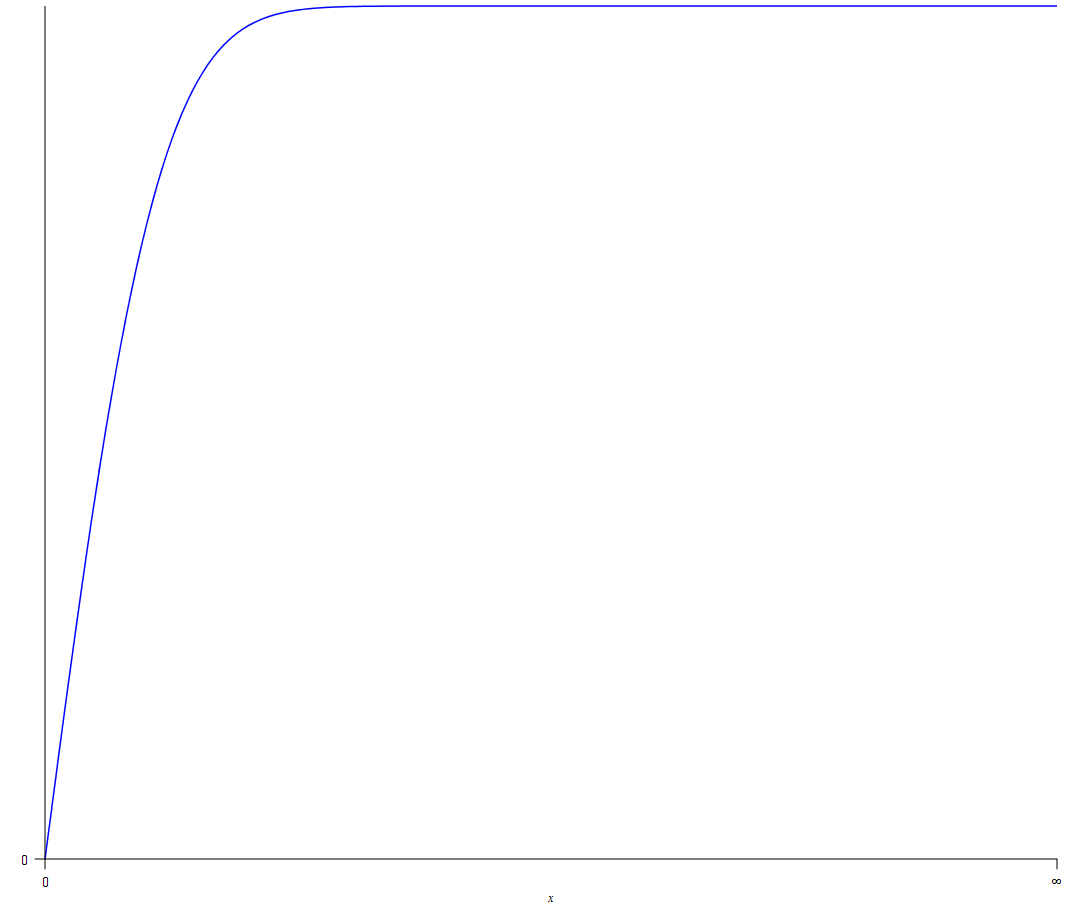
\includegraphics[scale = 0.15]{erf}
\caption{The error function, $\erf(x), 0 < x < \infty$}
\label{fig:erf}
\end{figure}

so our solution can be rewritten as:\bigskip

\begin{eqnarray*}  
  f(z) & = & \sqrt{\pi} c_1 \erf \left( \frac{z}{2} \right) + c_2 \\\\
       & = & C_1 \erf \left( \frac{z}{2} \right) + C_2
\end{eqnarray*}\medskip

and our final solution is:\bigskip

\[ u(x, t) = C_1 \erf \left( \frac{x}{\sqrt{4 \alpha t}} \right) + C_2 \]\medskip









\chapter{The Freezing Problem}



\section{The One-Phase Stefan Problem}

To begin lets take a simple problem - that of a semi-infinite region $0 < x < \infty$ within which liquid 
freezes. Let us assume that the liquid freezes from left to right, with a solidification front $x = s(t)$. 
Let $u(x, t)$ be the temperature of the solidified water (ice). Assume the initial temperature of the 
liquid is at $0^{\circ}\mathrm{C}$, and the temperature on the left boundary is kept at 
$-1^{\circ}\mathrm{C}$ (just below freezing). We can describe our system with the following equations:\bigskip

\begin{eqnarray*} 
  \frac{\partial u}{\partial t} & = & \alpha \frac{\partial^2 u}{\partial x^2}, \qquad 0 < x < s(t), \qquad t > 0 \\\\
                        u(0, t) & = & -1 \\
                     u(s(t), t) & = & 0 
\end{eqnarray*}\medskip

where $\alpha$ is the diffusivity. As we don't know the nature of $s(t)$ - the solidification front - we 
need another condition to help us find it. This boundary condition, a \emph{Stefan Condition},  we have 
discussed in detail in the previous chapter. So we add two more conditions to our system of equations:\bigskip

\begin{eqnarray*} 
  k \frac{\partial u}{\partial x} (s(t), t) & = & \lambda \rho \frac{d s}{d t} \\\\
                                       s(0) & = & 0 
\end{eqnarray*}\medskip

where $\lambda$ in this case is the specific latent heat of fusion for water. Our similarity solution to 
the heat equation we found to be:\bigskip

\[ u(x, t) = C_1 \erf \left( \frac{x}{\sqrt{4 \alpha t}} \right) + C_2 \]\medskip

We need to find $C_1$ and $C_2$. To do this, lets first assume all constants are equal to 1:\bigskip

\[ \alpha = \lambda = \rho = k = 1 \]\medskip

By using our boundary condition $u(s(t), t) = 0$ we get:\bigskip

\begin{eqnarray*}
  C_1 \erf \left( \frac{s(t)}{2 \sqrt{t}} \right) + C_2 & = & 0 \\\\
            \erf \left( \frac{s(t)}{2 \sqrt{t}} \right) & = & - \frac{C_2}{C_1}
\end{eqnarray*}\medskip

which implies that $\frac{s(t)}{2 \sqrt{t}}$ must be a constant.\bigskip

\begin{figure}[b]
\centering
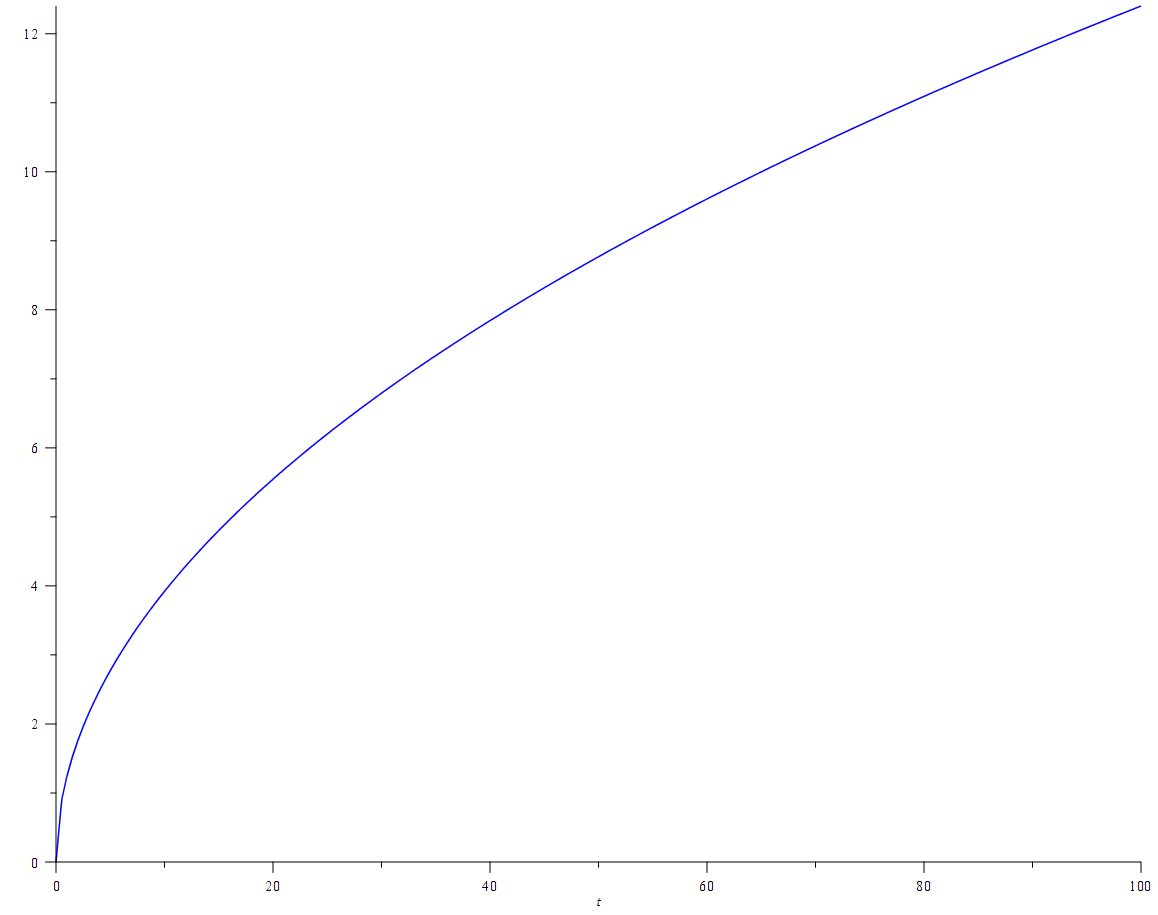
\includegraphics[scale = 0.15]{s-vs-t}
\caption{The moving boundary $s(t)$}
\label{fig:s-vs-t}
\end{figure}

\begin{eqnarray*}
  \frac{s(t)}{2 \sqrt{t}} & = & m \\\\
                     s(t) & = & 2 m \sqrt{t}
\end{eqnarray*}\medskip

Using our other boundary condition $u(0, t) = -1$, and with $\erf ( 0 ) = 0$, we get for $C_2$:\bigskip

\begin{eqnarray*}
  C_1 \erf ( 0 ) + C_2 & = & -1 \\
                   C_2 & = & -1
\end{eqnarray*}\medskip

solving for $C_1$:\bigskip

\begin{eqnarray*}
  C_1 \erf (m) - 1 & = & 0 \\\\
               C_1 & = & \frac{1}{\erf(m)}
\end{eqnarray*}\medskip

putting $C_1$ and $C_2$ back into our solution for $u(x, t)$:\bigskip

\[ u(x, t) = \frac{ \erf ( x / 2 \sqrt{t} ) }{\erf(m)} - 1 \]\medskip

Now we substitute our solution for $u(x, t)$ into the Stefan condition in order to find the unknown $m$:\bigskip

\[ \frac{\partial u}{\partial x} (s(t), t) = \frac{d s}{d t} \]\medskip

beginning with the LHS:\bigskip

\begin{eqnarray*} 
\frac{\partial u}{\partial x} & = & \frac{1}{\erf(m)} \cdot \frac{ \partial }{ \partial x } \Bigg[ \erf \left( \frac{x}{2 \sqrt{t}} \right) \Bigg] \\\\
                              & = & \frac{1}{\erf(m)} \cdot \frac{1}{ 2 \sqrt{t} } \cdot \frac{2}{ \sqrt{\pi} } \cdot e^{-(\sfrac{x}{2 \sqrt{t}})^2} \\\\
                              & = & \frac{1}{\erf(m)} \cdot \frac{1}{ \sqrt{\pi t} } \cdot e^{-(\sfrac{x}{2 \sqrt{t}})^2} 
\end{eqnarray*}\medskip

evaluated at $x = s(t)$:\bigskip

\begin{eqnarray*} 
\frac{\partial u}{\partial x} (s(t), t) & = & \frac{1}{\erf(m)} \cdot \frac{1}{ \sqrt{\pi t} } \cdot e^{-(\sfrac{s(t)}{2 \sqrt{t}})^2} \\\\
                                        & = & \frac{1}{\erf(m)} \cdot \frac{1}{ \sqrt{\pi t} } \cdot e^{-m^2} 
\end{eqnarray*}\medskip

moving to the RHS:\bigskip

\begin{eqnarray*}
           s(t) & = & 2 m \sqrt{t} \\
\frac{d s}{d t} & = & \frac{m}{ \sqrt{t} }
\end{eqnarray*}\medskip

\begin{figure}[b]
\centering
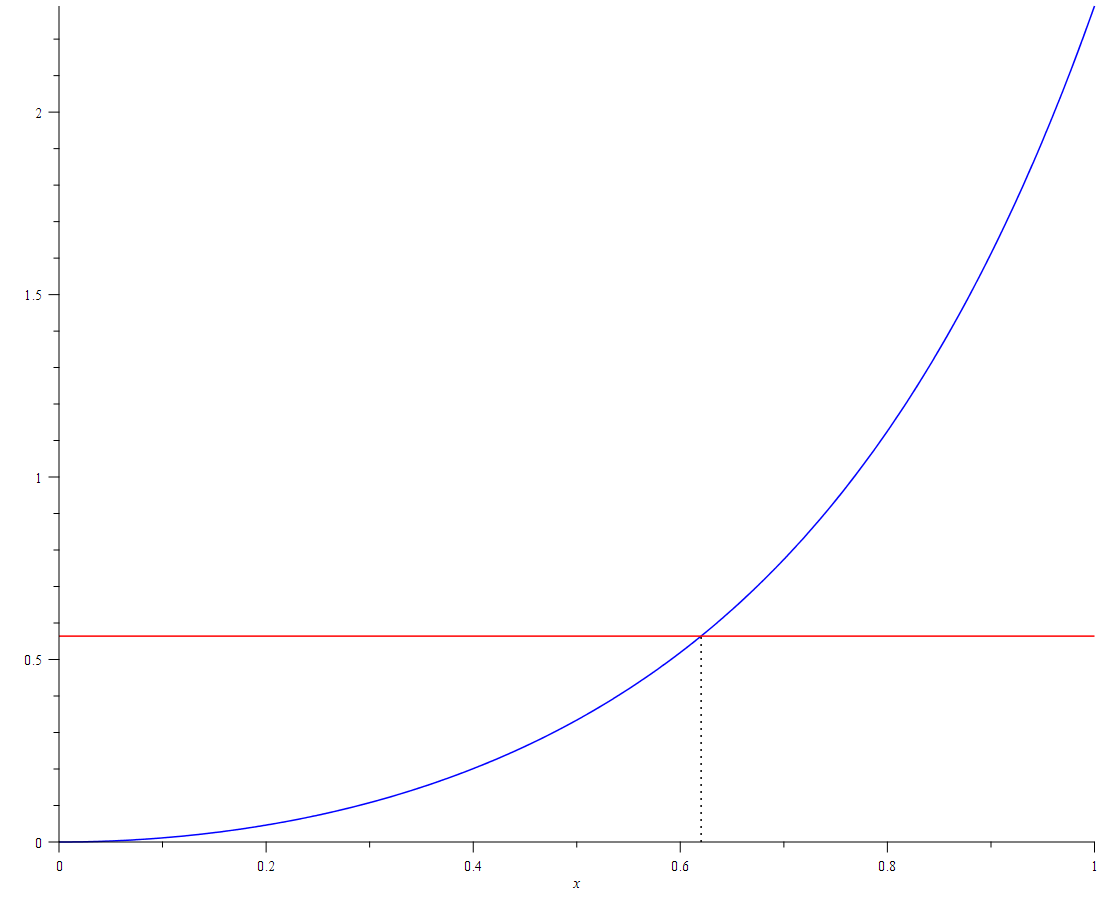
\includegraphics[scale = 0.15]{m-solved}
\caption{Solving for $m$ graphically}
\label{fig:m-solved}
\end{figure}

and finally equating the LHS and the RHS:\bigskip

\begin{eqnarray*}
\frac{1}{\erf(m)} \cdot \frac{1}{ \sqrt{\pi t} } \cdot e^{-m^2} & = & \frac{m}{ \sqrt{t} } \\\\
                                  m \cdot \erf(m) \cdot e^{m^2} & = & \frac{1}{ \sqrt{\pi} }
\end{eqnarray*}\medskip

which we can solve graphically (see figure \ref{fig:m-solved}) or numerically. Using Maple and the 
\emph{fsolve} function we find the numerical solution for $m$ to be $0.6201$ to $4$ decimal places.\bigskip

\begin{figure}[H]
\centering
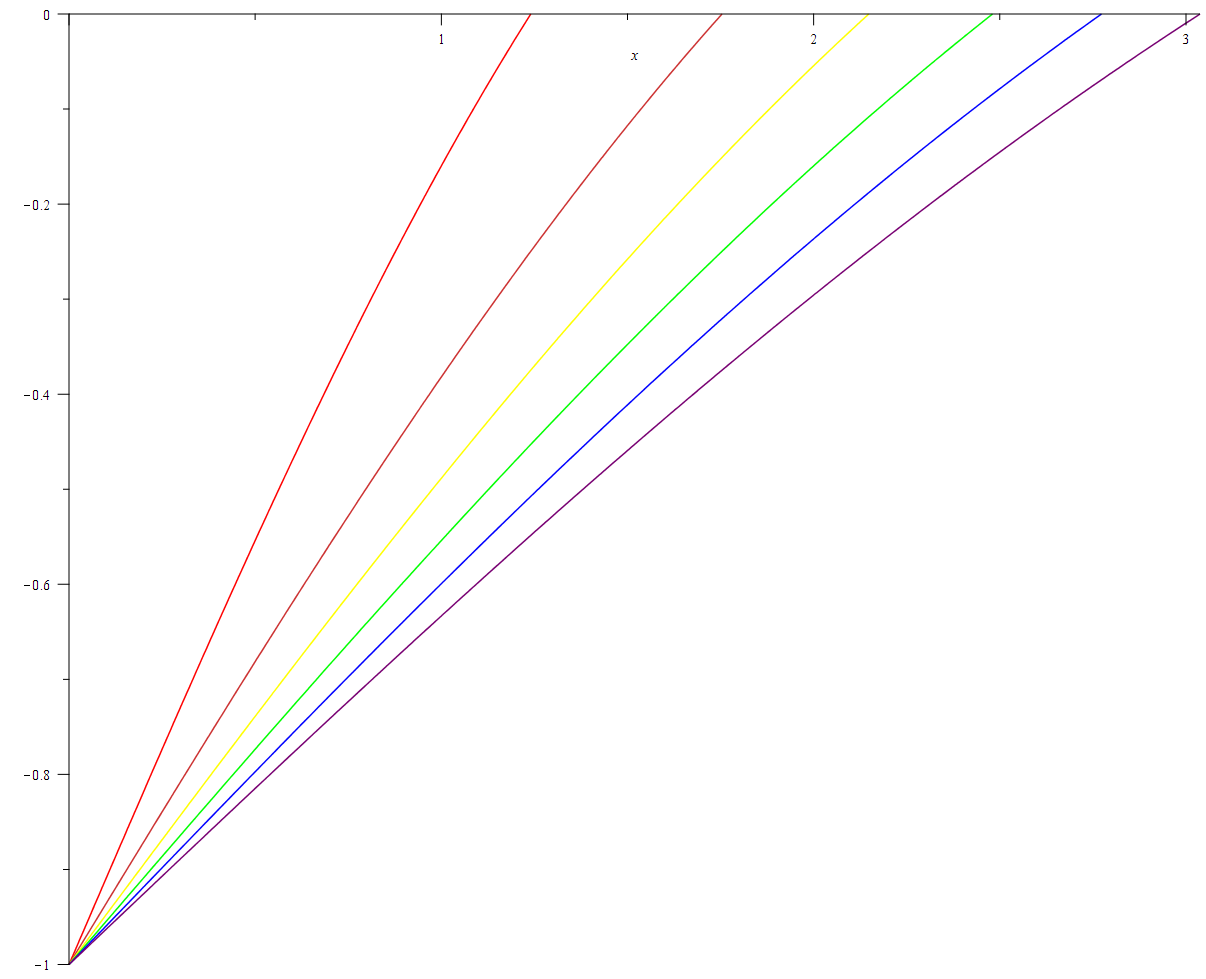
\includegraphics[scale = 0.15]{u-vs-x}
\caption{Temperature ($u$) for various different values of $x$}
\label{fig:u-vs-x}
\end{figure}

In figure \ref{fig:u-vs-x} we see a plot of the temperature $u$ for values of $x$ ranging from $1$ to $6$, 
and in figure \ref{fig:s-vs-t-contour} we see a contour plot of the temperature for differing values of $x$ 
and $t$, with temperature ranging from blue (colder) to grey (warmer).\bigskip

\begin{figure}[h]
\centering
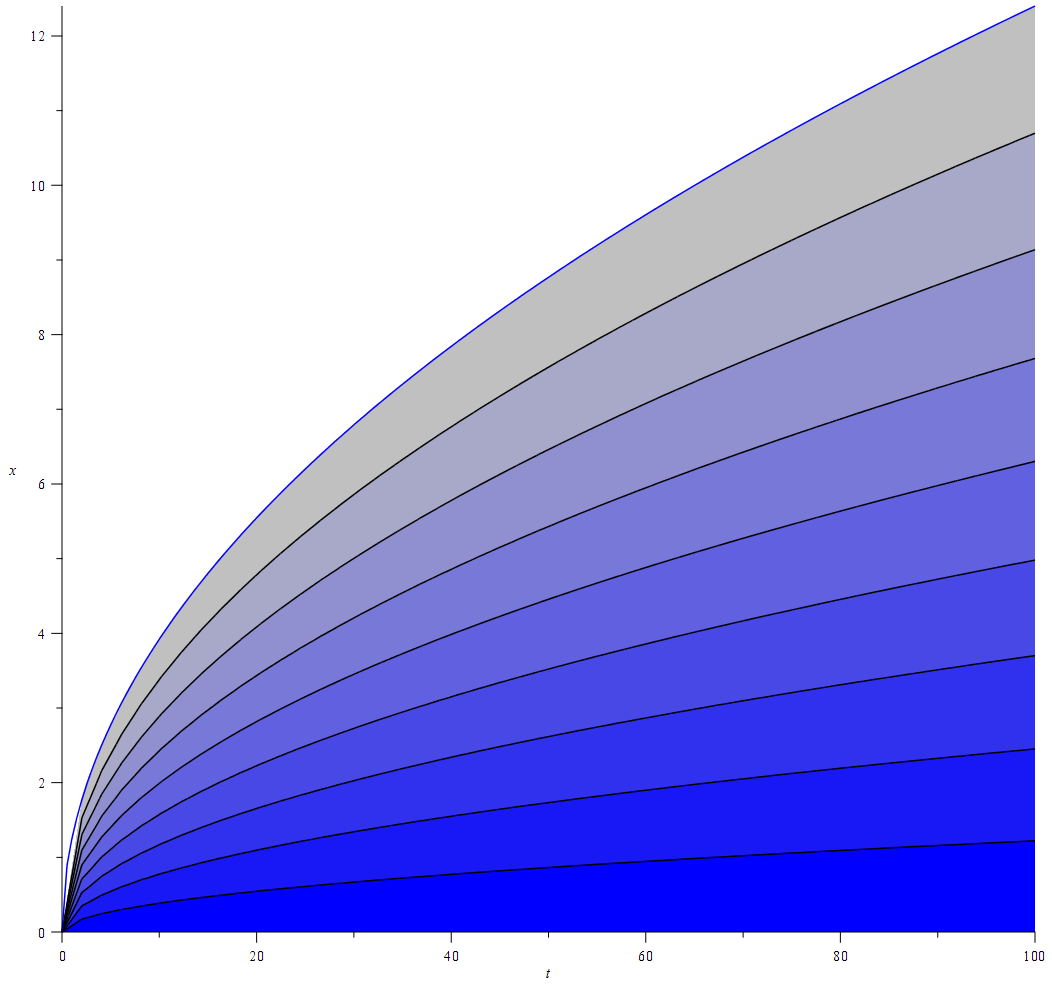
\includegraphics[scale = 0.15]{s-vs-t-contour}
\caption{A contour plot of Temperature ($u$) versus $x$ and $t$}
\label{fig:s-vs-t-contour}
\end{figure}










\section{The Pseudo-Steady-State Approximation Method}

The speudo-steady-state approximation method is a solution obtained under the assumption that the time 
derivative in the heat equation is negligible, and hence can be set to $0$. To re-state our freezing 
problem:\bigskip

\begin{eqnarray*} 
  \frac{\partial u}{\partial t} & = & \frac{\partial^2 u}{\partial x^2}, \qquad 0 < x < s(t), \qquad t > 0 \\\\
                        u(0, t) & = & -1 \\
                     u(s(t), t) & = & 0 
\end{eqnarray*}\medskip

with Stefan Condition:\bigskip

\begin{eqnarray*} 
  \frac{\partial u}{\partial x} (s(t), t) & = & \frac{d s}{d t} \\\\
                                       s(0) & = & 0 
\end{eqnarray*}\medskip

Under the assumption that the time derivative can be set to $0$, the heat equation reduces to:\bigskip

\[ \frac{\partial^2 u}{\partial x^2} = 0 \]\medskip

which can be solved easily:\bigskip

\begin{eqnarray*} 
  \frac{\partial^2 u}{\partial x^2} & = & 0 \\\\
      \frac{\partial u}{\partial x} & = & c_1(t) \\\\
                                  u & = & c_1(t) x + c_2(t) 
\end{eqnarray*}\medskip

and the constants of integration, $c_1$ and $c_2$ can be obtained readily using the boundary conditions. 
Our first boundary condition, $u(0, t) = -1$, gives us:\bigskip

\begin{eqnarray*} 
  c_1(t) \cdot 0 + c_2(t) & = & -1 \\
                   c_2(t) & = & -1
\end{eqnarray*}\medskip

and our second boundary condition, $u(s(t), t) = 0$, gives us:\bigskip

\begin{eqnarray*} 
  c_1(t) \cdot s(t) - 1 & = & 0 \\
                 c_1(t) & = & \frac{1}{s(t)}
\end{eqnarray*}\medskip

so our general solution for $u$ is:\bigskip

\[ u(x, t) = \frac{x}{s(t)} - 1 \]\medskip

it's first derivative with respect to $x$ is:\bigskip

\[ \frac{\partial u}{\partial x} = \frac{1}{s(t)} \]\medskip

and making use of the first Stefan Condition:\bigskip

\begin{eqnarray*} 
\frac{d s}{d t} & = & \frac{1}{s} \\\\
     s \cdot ds & = & dt \\\\
\int s \cdot ds & = & \int dt \\\\
  \frac{s^2}{2} & = & t + c \\\\
              s & = & \sqrt{2 t} + C
\end{eqnarray*}\medskip

and using the second Stefan Condition, $s(0) = 0$, we get:\bigskip

\begin{eqnarray*} 
\sqrt{2 \cdot 0} + C & = & 0 \\
                   C & = & 0 
\end{eqnarray*}\medskip

which gives us:\bigskip

\begin{eqnarray*} 
   s(t) & = & \sqrt{2 t} \\
u(x, t) & = & \frac{x}{\sqrt{2 t}} - 1 
\end{eqnarray*}\medskip

\begin{figure}[t]
\centering
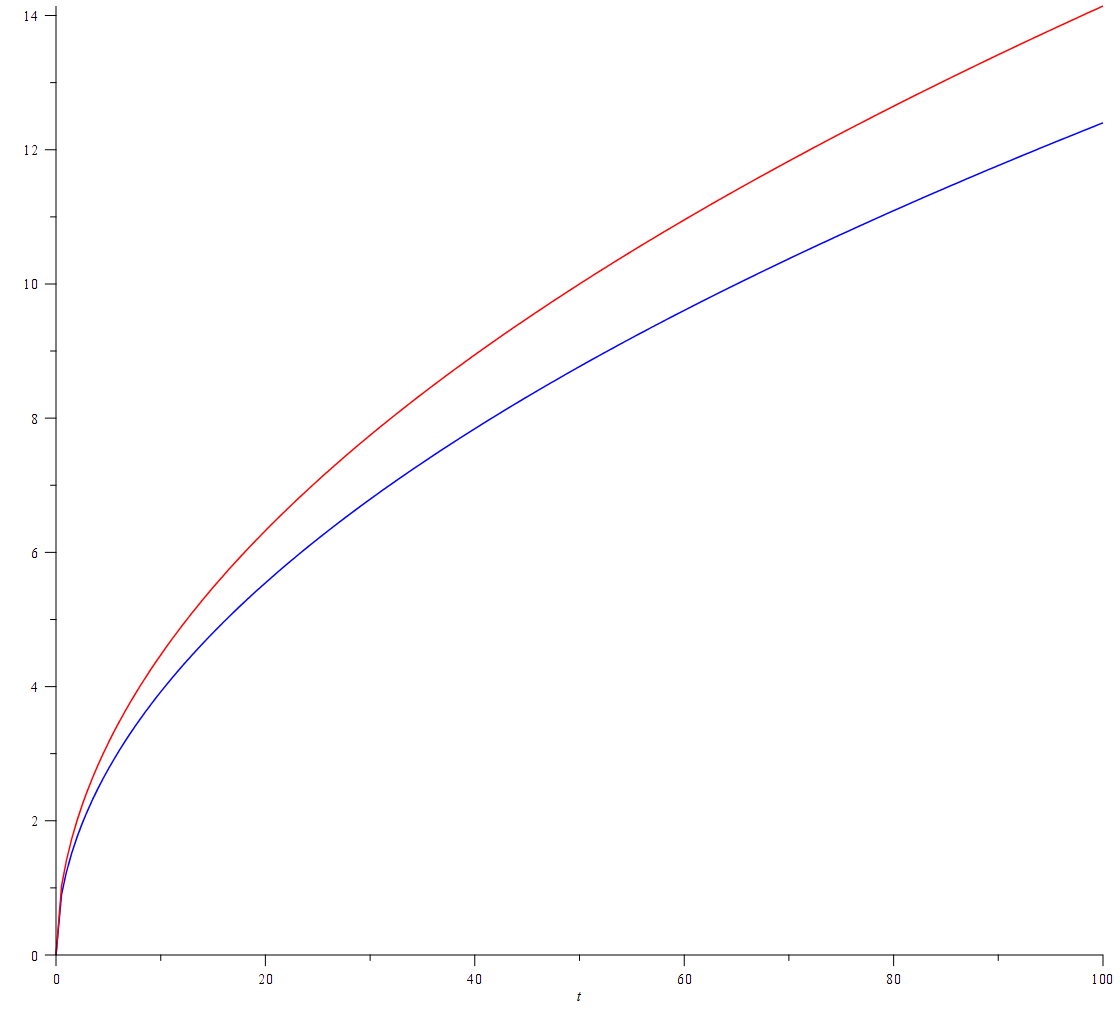
\includegraphics[scale = 0.15]{s-exact-vs-approximate}
\caption{A plot of the exact (blue) versus approximate (red) solutions for $s$}
\label{fig:s-exact-vs-approximate}
\end{figure}

\begin{figure}[b]
\centering
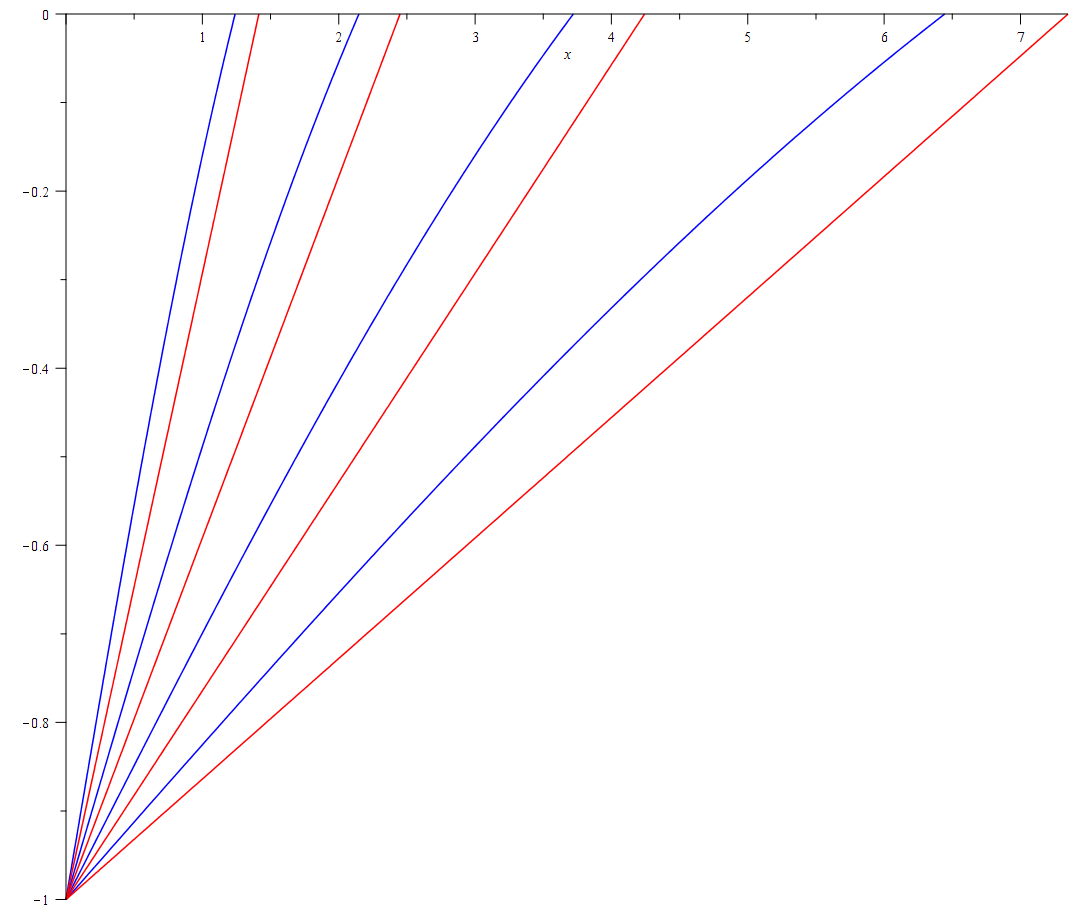
\includegraphics[scale = 0.15]{u-exact-vs-approximate}
\caption{A plot of the exact (blue) versus approximate (red) solutions for $u$}
\label{fig:u-exact-vs-approximate}
\end{figure}

So how does this approximation compare with the exact solution previously discussed? Looking at figure 
\ref{fig:s-exact-vs-approximate}, which plots the exact versus approximate solution for $s$, we can see 
they are reasonably close.\bigskip

But what about $u$? In figure \ref{fig:u-exact-vs-approximate}, which plots the exact versus approximate 
solution for $u$ for a number of different values of time, we can see that they are also reasonably close. 
In both cases the approximation is not perfect, but is certainly an acceptable approximation for drawing 
conclusions about the behaviour of the modelled system.
















\section{The Two-Phase Stefan Problem}

In the previous approach we solved for the moving boundary and the temperature of the solid region behind 
the moving boundary. We were not concerned with the temperature of the water.\bigskip

We will now consider a Two-Phase Stefan Problem - one where the temperatures of both phases are considered. 
We will reformulate our problem slightly:\bigskip

\begin{eqnarray*} 
  \frac{\partial u_S}{\partial t} & = & \alpha_S \frac{\partial^2 u_S}{\partial x^2}, \qquad 0 < x < s(t), \qquad t > 0 \\\\
  \frac{\partial u_L}{\partial t} & = & \alpha_L \frac{\partial^2 u_L}{\partial x^2}, \qquad s(t) < x < \infty, \qquad t > 0 \\\\
                        u_S(0, t) & = & u_1 \\
                     u_S(s(t), t) & = & 0 \\
                     u_L(s(t), t) & = & 0 \\
                        u_L(x, 0) & = & u_0 
\end{eqnarray*}\medskip

where $u_S$ is the temperature in the solid region, $u_L$ is the temperature in the liquid region, $u_1$ is 
the temperature on the left boundary, $u_0$ is the initial temperature of the liquid phase, and $\alpha_S, 
\alpha_L$ are the diffusivities of the solid and liquid regions respectively.\bigskip

The Stefan condition is as follows:\bigskip

\[
  -k_L \frac{\partial u_L}{\partial x} (s(t), t) + k_S \frac{\partial u_S}{\partial x} (s(t), t) = \rho \lambda \frac{d s}{d t} 
\]\medskip

We will use the similarity solution for the heat equation:\bigskip

\begin{eqnarray*}  
  u_S(x, t) & = & C_1 \erf \left( \frac{x}{\sqrt{4 \alpha_S t}} \right) + C_2 \\\\
  u_L(x, t) & = & C_3 \erf \left( \frac{x}{\sqrt{4 \alpha_L t}} \right) + C_4
\end{eqnarray*}\medskip

By using our boundary condition $u_S(s(t), t) = 0$ we get:\bigskip

\begin{eqnarray*}
  C_1 \erf \left( \frac{s(t)}{\sqrt{4 \alpha_S t}} \right) + C_2 & = & 0 \\\\
            \erf \left( \frac{s(t)}{\sqrt{4 \alpha_S t}} \right) & = & - \frac{C_2}{C_1}
\end{eqnarray*}\medskip

which implies that $\frac{s(t)}{\sqrt{4 \alpha_S t}}$ must be a constant.\bigskip

\begin{eqnarray*}
  \frac{s(t)}{\sqrt{4 \alpha_S t}} & = & m \\\\
                              s(t) & = & m \sqrt{4 \alpha_S t}
\end{eqnarray*}\medskip



We need to find $C_1, C_2, C_3,$ and $C_4$. Starting with $u_S$ and using our boundary condition 
$u_S(0, t) = u_1$:\bigskip

\begin{eqnarray*} 
  C_1 \erf \left( \frac{0}{\sqrt{4 \alpha_S t}} \right) + C_2 & = & u_1 \\\\
                                           C_1 \erf (0) + C_2 & = & u_1 \\
                                            C_1 \cdot 0 + C_2 & = & u_1 \\
                                                          C_2 & = & u_1 
\end{eqnarray*}\medskip

returning to our boundary condition $u_S(s(t), t) = 0$ we get:\bigskip

\begin{eqnarray*}
  C_1 \erf (m) + C_2 & = & 0 \\
                 C_1 & = & - \frac{C_2}{\erf(m)} \\\\
                     & = & - \frac{u_1}{\erf(m)} 
\end{eqnarray*}\medskip

so $u_S$ can be written:\bigskip

\begin{eqnarray*}
  u_S(x, t) & = & u_1 - \frac{u_1}{\erf(m)} \cdot \erf \left( \frac{x}{\sqrt{4 \alpha_S t}} \right) \\\\
            & = & u_1 \Bigg[ 1 - \frac{\erf ( x / \sqrt{4 \alpha_S t} )}{\erf(m)}  \Bigg] 
\end{eqnarray*}\medskip



Next $u_L$, and by using our boundary condition $u_L(x, 0) = u_0$ we get:\bigskip

\begin{eqnarray*} 
  C_3 \erf \left( \frac{x}{\sqrt{4 \alpha_L 0}} \right) + C_4 & = & u_0 \\\\
                                    C_3 \erf ( \infty ) + C_4 & = & u_0 \\
                                            C_3 \cdot 1 + C_4 & = & u_0 \\
                                                    C_3 + C_4 & = & u_0 
\end{eqnarray*}\medskip

and using our boundary condition $u_L(s(t), t) = 0$ we get:\bigskip

\begin{eqnarray*}
                   C_3 \erf \left( \frac{s(t)}{\sqrt{4 \alpha_L t}} \right) + C_4 & = & 0 \\\\
  C_3 \erf \left( \frac{m \sqrt{4 \alpha_S t}}{\sqrt{4 \alpha_L t}} \right) + C_4 & = & 0 \\\\
                 C_3 \erf \left( m \sqrt{\frac{\alpha_S}{\alpha_L}} \right) + C_4 & = & 0 
\end{eqnarray*}\medskip

and by using the fact that $C_3 + C_4 = u_0$ we can find $C_3$:\bigskip

\begin{eqnarray*}
      C_3 \erf \left( m \sqrt{\frac{\alpha_S}{\alpha_L}} \right) + C_4 & = & 0 \\\\
C_3 \erf \left( m \sqrt{\frac{\alpha_S}{\alpha_L}} \right) + u_0 - C_3 & = & 0 \\\\
                                                                   u_0 & = & C_3 - C_3 \erf \left( m \sqrt{\frac{\alpha_S}{\alpha_L}} \right) \\\\ 
                                                                       & = & C_3 \Bigg[ 1 - \erf \left( m \sqrt{\frac{\alpha_S}{\alpha_L}} \right) \Bigg] \\\\
                                                                   C_3 & = & \frac{u_0}{1 - \erf \left( m \sqrt{ \alpha_S / \alpha_L} \right)} 
\end{eqnarray*}\medskip

from which we can find $C_4$:\bigskip

\begin{eqnarray*}
  C_4 & = & -C_3 \erf \left( m \sqrt{\frac{\alpha_S}{\alpha_L}} \right) \\\\
  C_4 & = & -\frac{u_0 \erf ( m \sqrt{ \alpha_S / \alpha_L } )}{1 - \erf ( m \sqrt{ \alpha_S / \alpha_L } )} 
\end{eqnarray*}\medskip

so $u_L$ can be written:\bigskip

\begin{eqnarray*}
  u_L(x, t) & = & \frac{u_0 \erf ( x / \sqrt{4 \alpha_L t} )}{1 - \erf ( m \sqrt{ \alpha_S / \alpha_L} )} - \frac{u_0 \erf ( m \sqrt{\alpha_S / \alpha_L} )}{1 - \erf ( m \sqrt{\alpha_S / \alpha_L} )} \\\\
            & = & u_0 \Bigg[ 1 - \frac{1 - \erf ( x / \sqrt{4 \alpha_L t} )}{1 - \erf ( m \sqrt{\alpha_S / \alpha_L} )}  \Bigg] 
\end{eqnarray*}\medskip




Now we use the Stefan condition in order to find the unknown $m$. We first calculate the following derivatives:\bigskip

\begin{eqnarray*}
\frac{\partial u_S}{\partial x}(s(t), t) & = & \frac{u_1 e^{-m^2}}{\erf(m) \sqrt{\pi \alpha_S t}} \\\\
\frac{\partial u_L}{\partial x}(s(t), t) & = & \frac{u_0 e^{-( m \sqrt{\sfrac{\alpha_S}{\alpha_L}} )^2}}{( 1 - \erf ( m \sqrt{ \alpha_S / \alpha_L} ) ) \sqrt{\pi \alpha_L t}} \\\\
\frac{d s}{d t} & = & m \sqrt{\frac{\alpha_S}{t}}
\end{eqnarray*}\medskip

and then we substitute these into the Stefan condition, which gives us:\bigskip

\[
- k_L \left( \frac{u_0 e^{-( m \sqrt{\sfrac{\alpha_S}{\alpha_L}} )^2}}{( 1 - \erf ( m \sqrt{ \alpha_S / \alpha_L} ) ) \sqrt{\pi \alpha_L t}} \right) - k_S \left( \frac{u_1 e^{-m^2}}{\erf(m) \sqrt{\pi \alpha_S t}} \right) = \rho \lambda m \sqrt{\frac{\alpha_S}{t}}
\]\medskip

which can be solved numerically using maple.
















\chapter{The Continuous Casting Problem}



\section{Description}

We are interested in modelling a method that produces steel sheets by pouring molten steel onto a 
water-cooled rotating drum. As the molten steel hits the cooled drum it begins to cool and solidify. As it 
cools a "puddle" is formed from where the molten steel first comes into contact with the drum to where it 
has fully solidified. In order for this process to be successful, the puddle must disappear before the 
sheet is removed from the drum.\bigskip

The thickness of the sheets would be controlled by varying the rate of flow of the molten steel. If the 
steel sheets cool and solidify quickly enough they can be removed and further processed.\bigskip

We will now attempt to model this problem. Our approach will be to try to find the length of the puddle. 
For a drum rotating with speed $V$ the length of the puddle is simply:\bigskip

\[ \ell = V t_h \]\medskip

where $t_h$ is the time taken for the molten steel to solidify to a thickness $h$. What we are really 
interested in is the quantiy $t_h$. To find this time we can take a similar approach to the freezing 
problem previously discussed and treat this problem as a one-dimensional problem where the solidification 
boundary moves from the surface of the cooled drum to the extent of the molten metal. 










\section{Solution}

Let $u_1(x, t)$ denote the temperature of the drum, and let $u_2(x, t)$ 
denote the temperature of the solidified steel. And let $x = s(t)$ be the moving boundary between the 
solidified steel and the molten steel.\bigskip

\begin{eqnarray*} 
  \frac{\partial u_1}{\partial t} & = & \alpha_1 \frac{\partial^2 u_1}{\partial x^2}, \qquad -\infty < x < 0 \\\\
  \frac{\partial u_2}{\partial t} & = & \alpha_2 \frac{\partial^2 u_2}{\partial x^2}, \qquad 0 < x < s(t) 
\end{eqnarray*}\medskip

where $\alpha_1$ and $\alpha_2$ are the diffusivities of the drum material and the solidified steel 
respectively. Our boundary conditions are:\bigskip

\begin{eqnarray*} 
  u_1(-\infty, t) & = & u_d \\
        u_1(0, t) & = & u_2(0, t) \\
     u_2(s(t), t) & = & u_f 
\end{eqnarray*}\medskip

where $u_d$ is the temperature at the core of the drum, $u_f$ is the temperature that molten steel 
solidifies. Our continuity of flux condition is:\bigskip

\[
  -k_1 \frac{\partial u_1}{\partial x}(0, t) = -k_2 \frac{\partial u_2}{\partial x}(0, t)
\]\medskip

which basically states that the heat flux in the drum is the same for the metal. $k_1$ and $k_2$ are the 
thermal conductivities for the drum material and the steel respectively. And finally, our Stefan condition 
is:\bigskip

\[
  k_2 \frac{\partial u_2}{\partial x} (s(t), t) = \rho_2 \lambda \frac{d s}{d t} 
\]\medskip

In order to turn this problem into two seperate problems that we can solve independantly, we introduce a 
new value, $U$, which is the temperature at the point of contact between the drum and the steel:\bigskip

\[
  u_1(0, t) = u_2(0, t) = U
\]\medskip

So we now have two problems. For the drum:\bigskip

\begin{eqnarray*} 
  \frac{\partial u_1}{\partial t} & = & \alpha_1 \frac{\partial^2 u_1}{\partial x^2}, \qquad -\infty < x < 0 \\\\
                  u_1(-\infty, t) & = & u_d \\
                        u_1(0, t) & = & U 
\end{eqnarray*}\medskip

and for the steel:\bigskip

\begin{eqnarray*} 
  \frac{\partial u_2}{\partial t} & = & \alpha_2 \frac{\partial^2 u_2}{\partial x^2}, \qquad 0 < x < s(t)  \\\\
                     u_2(s(t), t) & = & u_f \\
                        u_2(0, t) & = & U 
\end{eqnarray*}\medskip

To solve this problem we will once again use the similarity solution for the heat equation:\bigskip

\begin{eqnarray*}  
  u_1(x, t) & = & C_1 \erf \left( \frac{x}{\sqrt{4 \alpha_1 t}} \right) + C_2 \\\\
  u_2(x, t) & = & C_3 \erf \left( \frac{x}{\sqrt{4 \alpha_2 t}} \right) + C_4
\end{eqnarray*}\medskip



By using our boundary condition $u_2(s(t), t) = u_f$ we see that:\bigskip

\begin{eqnarray*}
  C_3 \erf \left( \frac{s(t)}{\sqrt{4 \alpha_2 t}} \right) + C_4 & = & u_f \\\\
            \erf \left( \frac{s(t)}{\sqrt{4 \alpha_2 t}} \right) & = & \frac{u_f - C_4}{C_3}
\end{eqnarray*}\medskip

which once again implies that $\frac{s(t)}{\sqrt{4 \alpha_2 t}}$ must be a constant.\bigskip

\begin{eqnarray*}
  \frac{s(t)}{\sqrt{4 \alpha_2 t}} & = & m \\\\
                              s(t) & = & m \sqrt{4 \alpha_2 t}
\end{eqnarray*}\medskip



We need to find $C_1$, $C_2$, $C_3$, and $C_4$. Starting with $u_1$, and by using our boundary condition 
$u_1(0, t) = U$ we get:\bigskip

\begin{eqnarray*}
  C_1 \erf (0) + C_2 & = & U \\
                 C_2 & = & U
\end{eqnarray*}\medskip

and by using our boundary condition $u_1(-\infty, t) = u_d$ we get:\bigskip

\begin{eqnarray*}
  C_1 \erf (-\infty) + C_2 & = & u_d \\
                -C_1 + C_2 & = & u_d \\
                       C_1 & = &  C_2 - u_d \\
                           & = &  U - u_d 
\end{eqnarray*}\medskip

so now we have:\bigskip

\[ u_1(x, t) = U + (U - u_d) \erf ( x / \sqrt{4 \alpha_1 t} )  \]\medskip



Moving on to $u_2$, and by using our boundary condition $u_2(0, t) = U$ we get:\bigskip

\begin{eqnarray*}
  C_3 \erf (0) + C_4 & = & U \\
                 C_4 & = & U
\end{eqnarray*}\medskip

and again by using our boundary condition $u_2(s(t), t) = u_f$ we get:\bigskip

\begin{eqnarray*}
  C_3 \erf (m) + C_4 & = & u_f \\
                 C_3 & = & \frac{u_f - C_4}{\erf (m)} \\\\
                     & = & \frac{u_f - U}{\erf (m)} 
\end{eqnarray*}\medskip

so now we have:\bigskip

\[ u_2(x, t) = U + (u_f - U) \frac{\erf ( x / \sqrt{4 \alpha_2 t} )}{\erf (m)}  \]\medskip



All that remains is to solve for $U$ and $m$. We first calculate the following derivatives:\bigskip

\begin{eqnarray*}
  \frac{\partial u_1}{\partial x} & = & \frac{(U - u_d) e^{-(x / \sqrt{4 \alpha_1 t})^2}}{\sqrt{\pi \alpha_1 t}} \\\\
  \frac{\partial u_2}{\partial x} & = & \frac{(u_f - U) e^{-(x / \sqrt{4 \alpha_2 t})^2}}{\erf (m) \sqrt{\pi \alpha_2 t}} \\\\
                  \frac{d s}{d t} & = & m \sqrt{\frac{\alpha_2}{t}}
\end{eqnarray*}\medskip

and then we substitute into the remaining boundary conditions, starting with the continuity of flux:\bigskip

\begin{eqnarray*}
  -k_1 \frac{U - u_d}{\sqrt{\pi \alpha_1 t}} & = & -k_2 \frac{u_f - U}{\erf (m) \sqrt{\pi \alpha_2 t}} \\\\
                                     U - u_d & = & \frac{k_2}{k_1} \sqrt{\frac{\alpha_1}{\alpha_2}} \frac{u_f - U}{\erf (m)} \\\\
                                             & = & \beta \frac{u_f - U}{\erf (m)} \qquad \text{ where } \qquad \beta = \frac{k_2}{k_1} \sqrt{\frac{\alpha_1}{\alpha_2}} \\\\
                   U \erf (m) - u_d \erf (m) & = & u_f \beta - U \beta \\
                        U \erf (m) + U \beta & = & u_d \erf (m) + u_f \beta \\\\
                                           U & = & \frac{u_d \erf (m) + u_f \beta}{\erf (m) + \beta}
\end{eqnarray*}\medskip

followed by the Stefan condition:\bigskip

\begin{eqnarray*}
  k_2 \frac{(u_f - U) e^{-m^2}}{\erf (m) \sqrt{\pi \alpha_2 t}} & = & \rho_2 \lambda m \sqrt{\frac{\alpha_2}{t}} \\\\
                                             m e^{m^2} \erf (m) & = & \frac{k_2 (u_f - U)}{ \sqrt{\pi} \rho_2 \lambda \alpha_2 } 
\end{eqnarray*}\medskip

and from our solution for $U$ we have:\bigskip

\begin{eqnarray*}
           \beta & = & \frac{(U - u_d)}{(u_f - U)} \erf (m) \\\\
 m e^{m^2} \beta & = & \frac{(U - u_d)}{(u_f - U)} m e^{m^2} \erf (m) \\\\
                 & = & \frac{(U - u_d)}{(u_f - U)} \frac{k_2 (u_f - U)}{ \sqrt{\pi} \rho_2 \lambda \alpha_2 } \\\\
                 & = & \frac{k_2 (U - u_d)}{ \sqrt{\pi} \rho_2 \lambda \alpha_2 } 
\end{eqnarray*}\medskip

adding the two gives us:\bigskip

\begin{eqnarray*}
 m e^{m^2} \erf (m)  + m e^{m^2} \beta & = & \frac{k_2 (u_f - U)}{ \sqrt{\pi} \rho_2 \lambda \alpha_2 } + \frac{k_2 (U - u_d)}{ \sqrt{\pi} \rho_2 \lambda \alpha_2 }  \\\\
                                       & = & \frac{k_2 (u_f - u_d)}{ \sqrt{\pi} \rho_2 \lambda \alpha_2 } \\\\
        m e^{m^2} (\erf (m)  + \beta ) & = & \sigma  \qquad \text{ where } \qquad \sigma = \frac{k_2 (u_f - u_d)}{ \sqrt{\pi} \rho_2 \lambda \alpha_2 } 
\end{eqnarray*}\medskip










\section{Results}

We are now in a position to calculate values for $U$, $m$, and a value for $t_h$, from which we can 
calculate the puddle length, $\ell$. As usual, we can solve for $m$ graphically (see figure 
\ref{fig:m-solved-cc}) or numerically.\bigskip

For our numerical calculation we will use the following values:\bigskip

\begin{figure}[t]
\centering
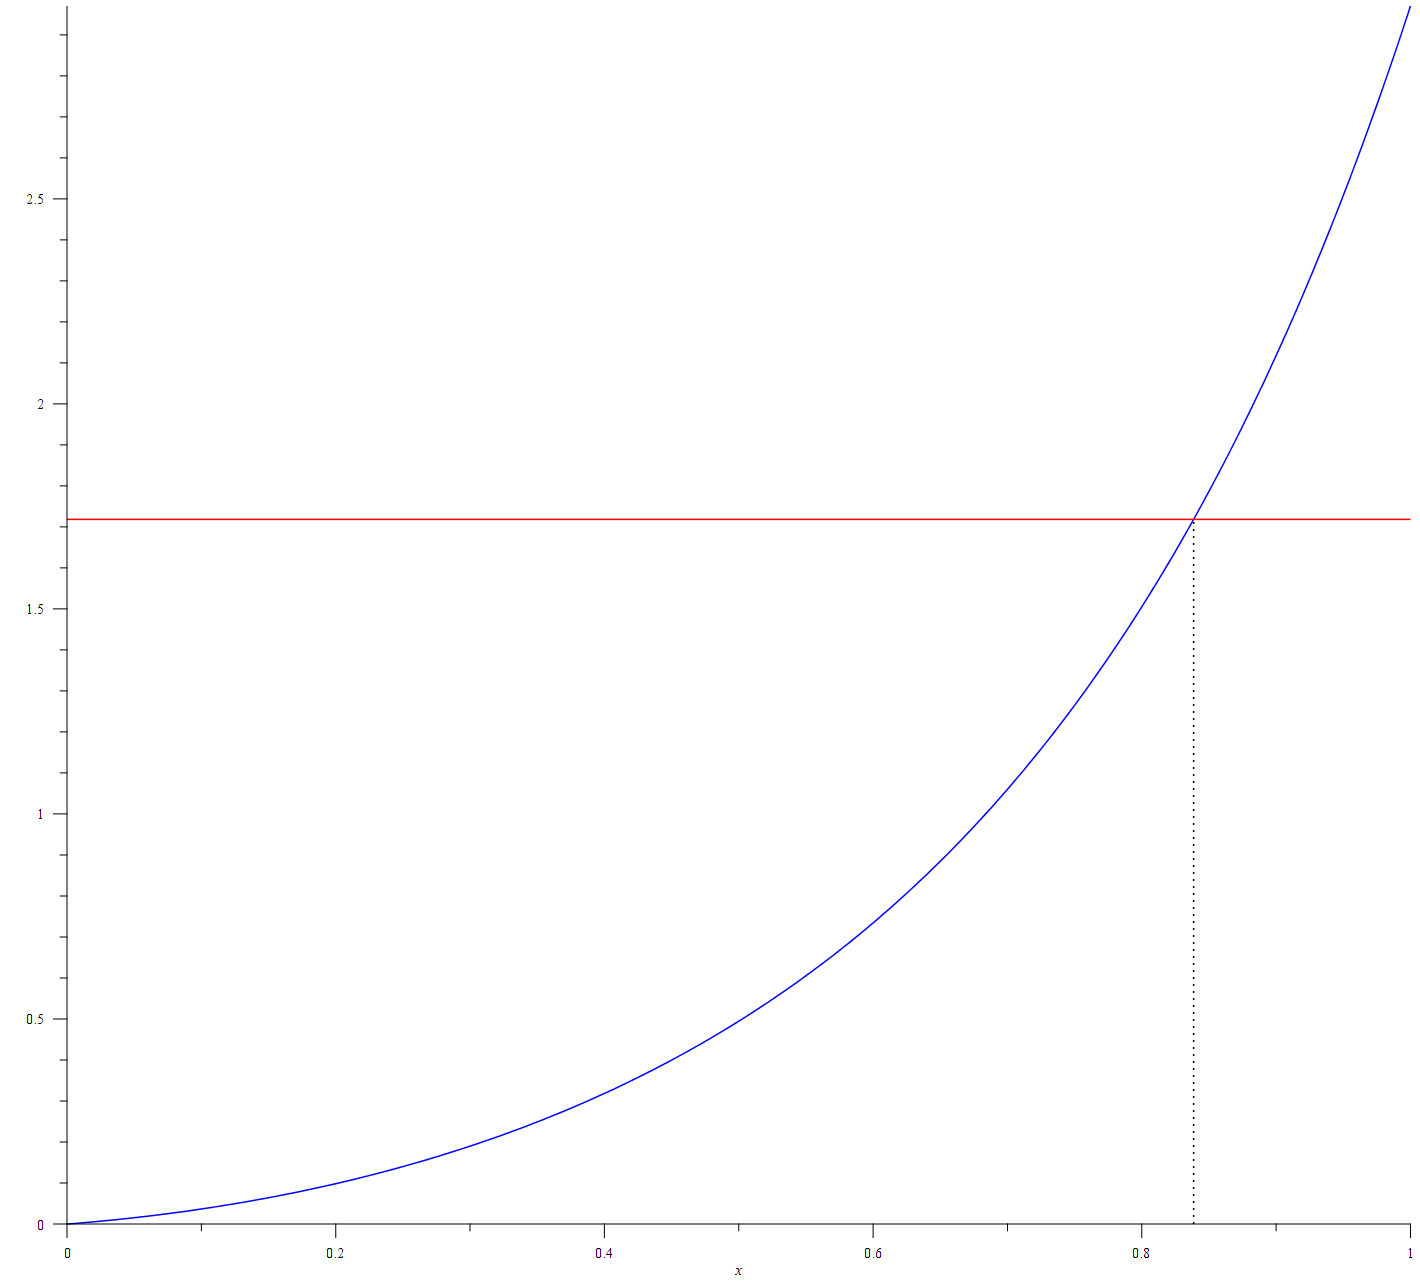
\includegraphics[scale = 0.15]{m-solved-cc}
\caption{Solving for $m$ graphically}
\label{fig:m-solved-cc}
\end{figure}

\begin{itemize}

\item $h$        \tab $0.01$ m

\item $V$        \tab $1$ m $s^{-1}$

\item $u_f$      \tab $1400^{\circ}\mathrm{C}$ 

\item $u_d$      \tab $150^{\circ}\mathrm{C}$ 

\item $\lambda$  \tab $2.7 \times 10^5$ J $kg^{-1}$

\item $\alpha_1$ \tab $10^{-4}$ $m^2 s^{-1}$

\item $\alpha_2$ \tab $4 \times 10^{-6}$ $m^2 s^{-1}$

\item $k_1$      \tab $400$ W $m^{-1 \circ}\mathrm{C}^{-1}$

\item $k_2$      \tab $20$ W $m^{-1 \circ}\mathrm{C}^{-1}$

\item $\rho_2$   \tab $7.6 \times 10^3$ kg $m^{-3}$

\end{itemize}\medskip

The material of the drum is chosen to be copper because of it's good conductivity. Using Maple and the 
\emph{fsolve} function we find the numerical solution for $U$, the teperature at the surface of the drum, 
to be $458.0798^{\circ}\mathrm{C}$ to $4$ decimal places, which is much less than the melting temperature 
of copper, which in turn is less than the melting temperature of steel. We find the numerical solution for 
$m$ to be $0.8386$ to $4$ decimal places. In order to calculate $t_h$ we find the time taken for the moving 
boundary to reach the thickness $h$:\bigskip

\begin{eqnarray*}
                   s(t_h) & = & h \\
  m \sqrt{4 \alpha_2 t_h} & = & h \\
    \sqrt{4 \alpha_2 t_h} & = & \frac{h}{m} \\\\
           4 \alpha_2 t_h & = & \frac{h^2}{m^2} \\\\
                      t_h & = & \frac{h^2}{4 \alpha_2 m^2} 
\end{eqnarray*}\medskip

from which we find the numerical solution to $t_h$ to be $8.8878$ seconds to $4$ decimal places. With a 
value for $V$ set to $1$ m $s^{-1}$, our puddle length $\ell$ is $8.8878$ metres to $4$ decimal places.

\begin{figure}[h]
\centering
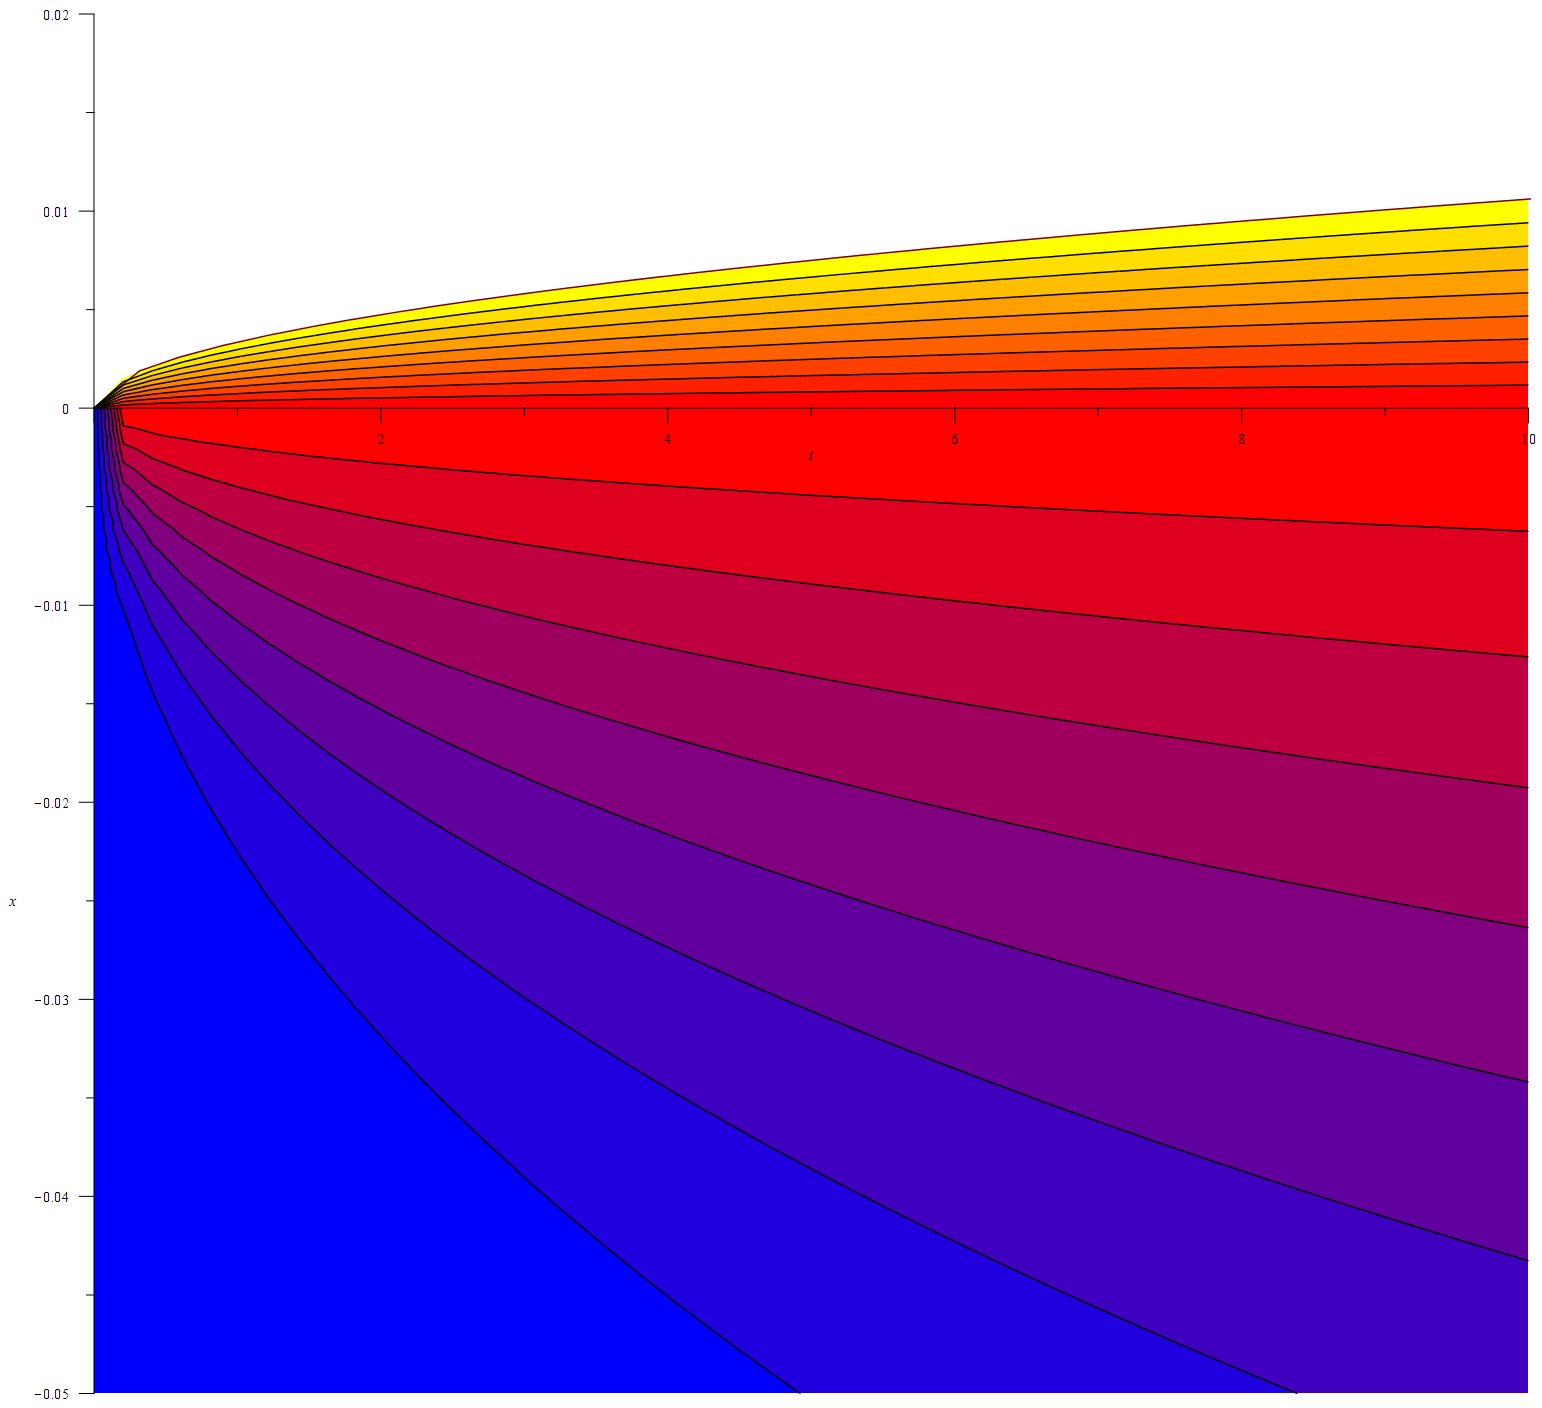
\includegraphics[scale = 0.15]{s-vs-t-contour-cc}
\caption{A contour plot of Temperature ($u$) versus $x$ and $t$}
\label{fig:s-vs-t-contour-cc}
\end{figure}

In figure \ref{fig:s-vs-t-contour-cc} we see a contour plot of the temperature for differing values of $x$ 
and $t$, with temperature ranging from blue (colder) to red (warmer) to yellow (warmest). We see that as 
time advances, the solidification front advances, the solid steel cools as it approaches the drum surface, 
and the temperature of the drum increases, but decreases from the surface inwards.\bigskip













\chapter{Conclusions}

The calculated value for the puddle length, almost $9$ metres, seems very large, especially in comparison 
with the thickness of the sheet, $0.01$ metres, and would require a drum of an impractical size to ensure 
the molten steel had solidified before leaving the drum, and for this reason the approach must be deemed 
unfeasible. On the other hand, the approach to modelling the problem itself seems to be successful.\bigskip








% ~\cite{logan2004applied}
% ~\cite{fulford2002industrial}





\bibliographystyle{plain}
\bibliography{bibtex/Applied_Partial_Differential_Equations,bibtex/Free_And_Moving_Boundary_Problems,bibtex/Industrial_Mathematics}{}


\end{document}
